%
% File main.tex
%
% Contact: car@ir.hit.edu.cn, gdzhou@suda.edu.cn
%%e.agirre@ehu.es or Sergi.Balari@uab.es
%% and that of ACL 08 by Joakim Nivre and Noah Smith

\documentclass[11pt]{article}
\usepackage{comment}
\usepackage{acl2015}
\setlength\titlebox{6cm}
\usepackage{times}
\usepackage{url}
\usepackage{hyperref}
\usepackage{latexsym}
\usepackage{biblatex}
\addbibresource{bibliography.bib}
\usepackage{csquotes}
\usepackage{tabularx}
\usepackage{xcolor}
\usepackage{svg}

\title{Music genre classification based on song lyrics - comparison between different word embedding techniques and classifiers \\Project Proposal for NLP Course, Winter 2022}

\author{Bartłomiej Eljasiak \\
  Warsaw University of Technology \\
  {\tt\small bartlomiej.eljasiak.stud@pw.edu.pl} \\\And
  Aleksandra Nawrocka \\
  Warsaw University of Technology \\
  {\tt\small aleksandra.nawrocka.stud@pw.edu.pl} \\
  \AND
  Dominika Umiastowska \\
  Warsaw University of Technology \\
  {\tt\small dominika.umiastowska.stud@pw.edu.pl} \\\And 
  supervisor: Anna Wróblewska\\
  Warsaw University of Technology \\
  {\tt\small anna.wroblewska1@pw.edu.pl}\\}

\date{}

\begin{document}
\raggedbottom

\maketitle

\vspace{5em}

\begin{abstract}

Music genre classification (MGC), although a well-known task, still remains challenging in the domain of Music Information Retrieval. We tackle the problem of MGC based solely on lyrics and try to solve it using a solution composed of a state-of-the-art word embedding method and a separate classification model. Our main contribution is the comparison between different word embedding methods and classification techniques, which in the domain of MGC is currently lacking. The novelty comes with an additional approach in the form of testing the impact of enriching the lyrics with the title of the song.

\end{abstract}



\section{Introduction}
A music genre is a conventional label on the musical piece which characterizes it as having certain features, conventions, or characteristics. It is quite a complicated problem to say precisely how genres are distinguished. The genre often dictates the style and rhythm of the audio of the song. It seems much harder to define the music genre by lyrics alone, even from a human perspective. Therefore, it is quite an interesting topic to try making such a distinction based on song text. Similar research has already been conducted, but this topic is yet to be fully explored.

The song's lyrics are often related to its melody and rhythm. It is also common for different genres to raise different topics. It was already shown that a combination of audio and text features gets better results than using only audio features \cite{mayer2011Ref}. Furthermore, lyrics may be more accessible and easier to process than audio. Therefore, lyrics classification seems to be an interesting field of study both for its own and for its potential connection with audio features.

We have previously explored different methods for lyrics-based genre classification. Our study included testing different methods of obtaining text embeddings, such as GloVe, word2vec, BERT, and varying classification models, such as Naive Bayes, Linear Support Vector Machine, XGBoost, and Convolutional Neural Network. In this research, we focus on improving obtained results. We add sentiment analysis for the classifier to see the lyrics from a different perspective. We build a model containing two separate models, where the first one decides whether the song belongs to the \textit{Rock} genre or not and the second one classifies samples into remaining genres. 

We also create a small dataset to explore using available APIs. Then we test some of the models on it.

The research paper is divided into multiple sections. In section \ref{related_work} we describe related works in the domain of MGC. Section \ref{approach} presents used datasets and the preprocessing done. Furthermore, used methods and models are characterized. In section \ref{hyperparameters} we show the hyperparameters of the models used. In section \ref{experiments} we demonstrate conducted experiments and obtained results. The whole project is concluded in section \ref{conclusion}.


\section{Related works}\label{related_work}

Music genre classification (MGC) is at this point a well-known research problem and a subdomain of Music Information Retrieval (MIR). Culture and therefore music avoids strict barriers and definitions, nevertheless, each piece of music is usually categorized into one or more genres. MGC enables us to study this categorization, explore similarities and differences between various genres or even construct a taxonomy. 

In the past, due to heavy computational limitations, the main focus of MGC was put on finding the best features for classification purposes. In \cite{oldFeatures} such features were e.g. \textit{AverageSyllablesPerWord} or \textit{SentenceLengthAverage}. Naturally, word embedding played an important role in extracting information from lyrics and the use of simple methods like \textit{bag-of-words} can be found in various papers \cite{mgc_example_1, liang2011music}. With time, an increasing amount of focus was put strictly on embeddings themselves, developing novel and improved representations. 

Currently, all state-of-the-art approaches for MGC utilizing lyrics rely heavily on word embeddings. In a recent publication \cite{musicWordEmbed} an attempt was made to train the embedding model strictly on lyrics. Unfortunately, the significance of the work is hard to assess due to the lack of usage of this model.

It is also rather common to approach MGC in a multi-modal manner. Usage of the audio itself has to be second if not the most popular source of information with many published articles \cite{audio_1dcnn, audio_attention, audio_reviews_cover, oldFeatures, oldAudio}. Other less trivial data sources are symbolic \cite{symbolic}, culture \cite{oldFeatures}, text reviews \cite{audio_reviews_cover}, and cover art \cite{audio_reviews_cover}. One could say that at this stage researchers experiment with enriching the pieces of music with any meaningful data possible.

The datasets that we work on are:
\begin{itemize}
    \item \textit{Song lyrics from 79 musical genres} dataset from Kaggle website \cite{KaggleDataset},
    \item \textit{MetroLyrics} dataset processed and put in a GitHub repository \cite{GithubDataset},
    \item our own dataset created using Spotify API \cite{Spotify} and Genius API \cite{Genius}.
\end{itemize}



\section{Approach and research methodology}

\subsection{Datasets}
While trying to find possible datasets for our project it was important to us for the song lyrics to be in their raw form. That means that they should not be transformed into e.g. bag-of-words model. The reason for this decision was that if we would like to use prepared models in a real-world scenario new song lyrics could be used with minimal preparation. What is more, as the language evolves all the time, with this approach there is still a possibility of further training of the models on song lyrics with the presence of not previously known words. And last but not least, we also wanted to minimize the risk of worse performance of prepared models which could be caused by simplifying the assumptions.

The effect of making this decision is the fact that we could not choose e.g. the musiXmatch dataset (the official lyrics collection of the Million Song Dataset \cite{Bertin-Mahieux2011}) as the dataset for conducting the experiments. This very well-known dataset consists of an enormous number of song lyrics which are unfortunately kept in a bag-of-words model form. But as we will not use this dataset, we also will not focus on its description.

We have found two datasets that meet our expectations:
\begin{itemize}
    \item \textit{Song lyrics from 79 musical genres} dataset from Kaggle website \cite{KaggleDataset},
    \item \textit{MetroLyrics} dataset processed and put in a GitHub repository \cite{GithubDataset}.
\end{itemize}

In the description of the first dataset, we can find the information that the dataset consists of 379 893 song lyrics from 4239 artists. Around 50\% of the song lyrics are in English and we will probably test our models on them. Information about the artists is kept in a separate file and contains a list of music genres each artist is connected with. As we plan to predict only one music genre for each song we will have to preprocess this dataset by reducing these lists to individual genres and assigning them to song lyrics of appropriate artists. Furthermore, song lyrics also need some preprocessing as they contain punctuation and span across multiple lines.

By contrast, the second dataset requires minimal work on our site. It was initially published on Kaggle website and consisted of 362 237 song lyrics from 18231 artists. The majority of song lyrics (probably around 60\%) were in English. Unfortunately, this dataset was removed from Kaggle website and we were not able to find it in its original form anywhere else. We have found a preprocessed version of it in a GitHub repository of a students' project performed by University of California students in 2018. This version's song lyrics have punctuation removed and contain only one genre for each entry. Based on descriptions of the original dataset we expect 11 genres and an unbalanced dataset with highly frequent \textit{Rock} label.

Finally, in case of problems connected to data we are considering creating our own dataset. This would be possible with the usage of Spotify API \cite{Spotify} and Genius API \cite{Genius}, which are well documented. We would use Spotify API to get recommendations of songs for chosen genres and Genius API for lyrics extraction. In comparison with both found datasets, our dataset would be a lot smaller but definitely balanced.

\subsection{Embeddings}

One of the key problems in the domain of natural language processing has to be the question of how to use words in a model which only understands numbers. This question sparked numerous attempts of representing language in a mathematical way. One can always assign each unique word a different number and in this way encode any language into the computer, but this is insufficient when it comes to using this encoded representation. It was rather clear, that in order for such transformation to be in any way useful, the original meaning of the word should be embedded into this numeric representation itself. This word embedding ought to be treated as a vector in a given, high-dimensional space. For a given model dimensionality is fixed, therefore each word is represented by a vector of a set length, typically a hundred or so numeric values.

There is still a task of creating a model capable of such transformations. It has a couple of possible approaches, mainly prediction-based and count-based. The second one, although simpler, will not be described here, since all methods described further make use of the first approach. Prediction-based word embedding models share a common trait, which unsurprisingly is that the embedding for a word was learned by performing the task of predicting given word \cite{baroni}. This definition does not set any requirements for the prediction itself, and, in fact, different approaches have been used successfully, such as the continuous Bag-of-Words Model (CBOW) and  continuous Skip-gram Model \cite{mikolov2013}.

There is a single more distinction for the different techniques used, which is significant for this work. The meaning of some words is not dependent on their structure or origin, but on the context in which they are used. In the case of homonyms, it is impossible to state the singular meaning of the word without context, e.g. bank as a financial institution vs. side of a river or play as in theatre vs. as in sport. More traditional embeddings do not incorporate the context of a word in determining its embedding. These models are called static or non-contextualized. The ones that do generate differentiable vectors depending on the context are subcategorized as contextualized word embeddings. Despite the described advantage of the latter method, prior has proven to be successful in multiple cases, such as GloVe \cite{glove} or fastText \cite{fastText}.

Other techniques which prove promising are ELMo \cite{elmo}, a deep bidirectional language model, which is pre-trained on a large text corpus and, extracting contextualized word embedding form, pre-trained Google’s Bidirectional Encoder Representations from Transformers (BERT) \cite{bert}. 

Little has been said about using word embedding in the context of music lyrics. \cite{musicWordEmbed} describes the process of training the word embedding model strictly on music lyrics, but lacks proper evaluation methods to be comparable to other works. This means that in order to reach state-of-the-art we are bound to testing various methods of word embedding, retraining them whenever it is possible. 



\subsection{Classification models}

We want to test a few varying classification models for this specific task. We will consider Naive Bayes classifier, Support Vector Machine, XGBoost, and Convolutional Neural Network.

Naive Bayes is a classifier based on Bayes' theorem known for good performance on real-world tasks despite being a simple model. It is fast and good at dealing with unbalanced data. It has also widespread applications on text classification tasks \cite{naiveBayesRef}.

Support Vector Machine tries to find a hyperplane that best separates samples of different classes. It is often used for text classification tasks and historically achieved great results \cite{svmRef}.

XGBoost \cite{xgboostRef} is a decision-tree based algorithm that uses a gradient boosting method. It shows great performance on large-scale tasks and is a very flexible and versatile tool.

Convolutional Neural Networks are one of the primarily used types of neural networks used commonly in both image and text classification \cite{cnnRef}. Their main feature is using layers with convolution filters that are applied to feature vectors.

As for CNN architecture, we want to test a few different optimizers, such as Adam optimizer \cite{adamRef}, Stochastic Gradient Descent and AdaDelta optimizer \cite{adadeltaRef}.

% Harris hawk nie bo nie ma gotowca zaimplementowanego w żadnej bibliotece więc pewnie będzie problem z użyciem tego

\subsection{Sentiment analysis}

It is a well-known fact that music can convey deep emotions to listeners. These emotions are present in both melody and lyrics. In this research, we decided to study the connection between those emotions contained in lyrics and the song genre. To do this we want to include sentiment analysis when classifying song lyrics to the song's genre. Since emotions in song lyrics are often non-binary we want to consider a model that can recognize more varying emotions.

We decided to use an already pre-trained model for emotion recognition called Emotion English DistilRoBERTa-base \cite{hartmann2022emotionenglish}.
The model was created by fine-tuning DistilRoBERTa-base and training it on the balanced dataset of $2800$ observations for each emotion summing up to 20k observations in total.

% Ten model ma accuracy 66% więc bez szału więc wolałam tego nie pisać...
% Na jego stronce jest jednak wypisane parę papierów które z niego korzystało więc fajnie że jest gdzieś faktycznie używany
% Inny z Hugging Face:
% https://huggingface.co/bhadresh-savani/bert-base-uncased-emotion
% Ten model ma niby wyższe accuracy ale jest to testowane na dziwnych datasetach więc nwm


The model predicts Ekman's six basic emotions, that is anger, disgust, fear, joy, sadness, surprise, and an additional neutral class - summing up to seven labels.

\subsection{Modified approach using sentiment analysis model and data fusion technique}

As mentioned above, besides comparing different word embedding techniques and classifiers, we want to test another, significantly modified approach. We want to take advantage of already existing, pre-trained sentiment analysis models and see if they can help to improve the accuracy of prepared architectures. To do that we will make use of methods known from multi-modal machine learning (of course we only have one modality).

The plan is to divide song lyrics in half. The first part will serve as an input to the word embedding model and the second to the sentiment analysis model. As outputs we will get an embedding of passed words and a vector of probabilities of different emotional states. These outputs, even though take the same form of numerical vectors, have different meanings. What is more, the output of the sentiment analysis model can be seen as a final decision as it contains information understandable to humans in contrast to the received embedding. However, the origins of these outputs may have common parts, e.g. reoccurring choruses, and because of that not as much information may be introduced in the second part of the song lyrics as would in the case of a new modality. Regardless of these considerations, we need to make use of data fusion techniques.

There are a lot of data fusion techniques. They can be divided into groups such as early fusion or late fusion. Early fusion is the process of merging data from multiple sources before conducting the analysis. This data can be described as input data, even though it is often already preprocessed, e.g. in the form of embeddings. An example of early fusion is simple concatenation of input data in the form of numerical vectors, where the resulting vector can be passed as input to the next module in the model's architecture. Late fusion is a concept similar to an ensemble. Classifiers are trained for all modalities and their outputs are merged to obtain a single decision e.g. by using weighted voting.

We are going to use an early fusion method even though part of our data will be in the final form. The method is called cross-modal attention \cite{Krishna2020MultimodalER} and is based on the usage of multi-head scaled dot product attention \cite{vaswani2017attention}. In contrast to self-attention, query matrix comes from a different modality than key and value matrices. This can help to capture relationships between different modalities. In our case, we will apply this method to only one modality by using the output of the sentiment analysis model for the query matrix and embedding of the first part of song lyrics for key and value matrices. This will lead to sentiment-guided lyrics feature output, which will be introduced as input data to a classifier.

We want to test if this approach will obtain better accuracy for the music genre classification problem. By using the sentiment analysis model and cross-modal attention mechanism we make our model more complex and introduce more trainable parameters. We also make use of transfer learning. These arguments weigh in favour of this approach. However, we only use the first halves of song lyrics to obtain embeddings and we do not introduce the second modality, even though we use a multi-modal data fusion technique, so predicted gains are lower than in the case of multiple modalities. As there exist arguments from both sides it is hard to tell what will be the outcome of the experiment.


\section{Experiments and results}\label{experiments}

\subsection{New models and embeddings}
 In this project, several embedding models were tested, but it was soon rather clear that the best results will be obtained by the most complex embedding models. Additionally, we wanted to decrease the input size of classifiers to reduce the training time and complexity of several models. Described goals were achieved by introducing new embedding models with aggregated word embeddings. Said models are \texttt{DistilBERT} and \texttt{SentenceTransformerMPNET} with word embeddings transformed to singular sentence embedding, by aggregating them. This seemingly minor change greatly increased accuracy scores across all classifiers and set a new standard for future experiments.

 We also used two new classifiers: DenseNet which consists of a few fully connected dense layers, and the 2-step CNN closer described before. 
 
 Results of our experiments on a balanced dataset are visible in \ref{tab:distilbert_results} and \ref{tab:mpnet_results} tables. $\Delta$ Acc. signify the difference between results acquired in this project for this dataset with the new embedding and the best results obtained in the previous project.

\begin{table}[!h]
\centering
\begin{tabular}{l|l|l|l}
\textbf{Classifier} & \textbf{Accuracy} & \textbf{F1-score} & \textbf{ $\Delta$ Acc.}  \\ \hline
NB         & 54.40\%           & 53.16\%           & + 11.16               \\
SVM          & 62.06\%           & 61.07\%           & + 11.45               \\
XGBoost             & 63.93\%           & 63.78\%           & \textbf{+ 18.46}      \\
\textbf{CNN}        & \textbf{65.47\%}  & \textbf{65.53\%}  & + 8.99                \\
DenseNet            & 64.96\%           & 64.99\%           & \multicolumn{1}{c}{-} \\
2StepCNN            & 62.21\%           & 57.97\%           & \multicolumn{1}{c}{-}
\end{tabular}
\caption{Results for the DistilBERT  on balanced dataset}
\label{tab:distilbert_results}
\end{table}

\begin{table}[!h]
\centering
\begin{tabular}{l|l|l|l}
\textbf{Classifier} & \textbf{Accuracy} & \textbf{F1-score} & \textbf{$\Delta$ Acc.}  \\ \hline
NB         & 56.23\%           & 55.97\%           & + 12.99               \\
SVM          & 62.83\%           & 61.66\%           & + 12.22               \\
XGBoost             & 62.45\%           & 62.31\%           & \textbf{+ 16.98}      \\
CNN                 & 65.06\%           & 64.30\%           & + 8.58                \\
\textbf{DenseNet}   & \textbf{66.42\%}  & \textbf{66.08\%}  & \multicolumn{1}{c}{-} \\
2StepCNN            & 63.34\%           & 60.44\%           & \multicolumn{1}{c}{-}
\end{tabular}
\caption{Results for the SentenceTransformerMPNET on balanced dataset}
\label{tab:mpnet_results}
\end{table}

As we can see, all results are significantly better than in the previous project which shows how important embedding is in text classification. Also, the new classifier DenseNet gives very good results, even given its quite simple structure. The comparison of the results is shown in Figure \ref{fig:embed_comparison}.

\subsection{Fine-tunning embedding models}
The natural next step was to improve the information contained in the embedding model by combining it with the classification layer and fine-tuning the combined architecture. Since a DistilBERT was pre-trained on a broad corpus and a wide range of texts, we hoped that by partially training it on lyrics it will be able to improve the quality of the created embeddings.  This task was realized on \texttt{small\_balanced} version of the available dataset. Unfortunately, repeated experiments did not bring the expected results and the model performance was not significantly improved. A comparison of both fine-tuned  and pre-trained models is presented in Table \ref{tab:tuning_results}. Lack of improvement may indicate problems in the training process but repeated experiments and tests on different models indicate that this was not the case. 


\begin{table}[h]
\centering
\begin{tabular}{l|r|r|r}
 \textbf{Embedding} & \textbf{Classifier} & \textbf{Accuracy} & \textbf{F1 score} \\\hline
pretrained & Dense & 0.6455 & 0.6431 \\
fine-tuned & Dense & \textbf{0.65} & \textbf{0.6682} \\
\end{tabular}
\caption{Results after fine-tuning}
\label{tab:tuning_results}
\end{table}

\subsection{Addition of sentiment analysis}
One of the main things that we wanted to test, was the impact of additional information added to the embeddings. At the same time since one of the assumptions of the project was working with only the lyrics, features that we could add to the embedding of the lyrics are all lyrics based. Our idea was to incorporate sentiment obtained by a separate model. Unfortunately, since we focused on using as hardware demanding embedding model there were little to no resources left for this sentiment model. After minor research we settled for \href{https://huggingface.co/gokuls/BERT-tiny-emotion-intent}{\texttt{BERT-tiny-emotion-intent}} model. It offers sentiment prediction in form of a six-dimensional vector measuring the sentiment as happy, sad, neutral, angry, excited, or frustrated. This is to some extent a redundancy since we expect the sentiment to be present in embeddings, at least to some degree, but this information may not be easy for the model to extract especially since our classification models are relatively simple.

We tested the influence of sentiment in two experiments. The first one was oriented on the changes in the performance of classifiers. As it can be seen in \ref{tab:sentiment_results} results for feature vector enriched with embeddings did not really change, when compared to \ref{tab:distilbert_results}. The only exception here is the XGBoost model which improved significantly, but this may be partially explained by the instability of the XGBoost which was observed. 

\begin{table}[h]
\centering
\begin{tabular}{l|r|r|r}
 \textbf{Classifier} & \textbf{Accuracy} & \textbf{Bal. Acc.} & \textbf{F1 score} \\\hline
Naive Bayes & 0.5272 & 0.5272 & 0.5095 \\
Linear SVM & 0.6054 & 0.6054 & 0.5998 \\
XGBoost & 0.6300 & 0.6300 & 0.6279 \\
CNN & 0.6433 & 0.6433 & \textbf{0.6433} \\
Dense & \textbf{0.6449} & \textbf{0.6449} & 0.6341 \\
\end{tabular}
\caption{Classification results for better embeddings }
\label{tab:sentiment_results}
\end{table}

The second experiment concerning sentiment included fine-tuning the combination of the embedding model, sentiment model and dense classifier. Same as with the previous first fine-tuning the results did not really change \ref{tab:sentiment_tuning_results}, and actually the model without sentiment achieves the best score, but only by a small margin of less than 1\%. 

\begin{table}[h]
\centering
\begin{tabular}{l|r|r}
 \textbf{sentiment}& \textbf{Accuracy} & \textbf{F1 score} \\\hline
yes &  0.6412 & 0.6638 \\
no &  \textbf{0.65} & \textbf{0.6682} \\
\end{tabular}
\caption{Results after fine-tuning with or without sentiment}
\label{tab:sentiment_tuning_results}
\end{table}

\subsection{Division into two models}

There were already shown some results for the 2-step CNN classifier on the balanced dataset in the previous section in tables \ref{tab:distilbert_results} and \ref{tab:mpnet_results}. In general, achieved by 2-step CNN accuracies were slightly worse than those of normal CNN and DenseNet.

But this classifier was created with the thought of an unbalanced dataset and therefore results on this dataset are the most important to us.  Therefore, we tested 2-step CNN and two other classifiers which gave the best results in previous tests on the unbalanced dataset (which is also much bigger than balanced) to see if separate recognition of the biggest class gives better results. Results are in Table \ref{tab:unbalanced_results_2_step} and the comparison is shown in Figure \ref{fig:metric_comparison}.

\begin{table}[!h]
\centering
\begin{tabular}{l|l|l|l}
\textbf{CLassifier} & \textbf{Accuracy} & \textbf{Bal. acc.} & \textbf{F1 score} \\ \hline
CNN                 & 64.74\%           & 50.71\%                & 60.88\%           \\
\textbf{NN}         & \textbf{65.23\%}  & 53.08\%                & \textbf{62.14\%}  \\
\textbf{2-step CNN} & 52.94\%           & \textbf{59.88\%}       & \textbf{54.11\%} 
\end{tabular}
\caption{Results for 2-step CNN, DenseNet, and CNN for DistilBERT on unbalanced dataset}
\label{tab:unbalanced_results_2_step}
\end{table}

Even though neither accuracy nor F1-score was better for 2-Step CNN, it proved to give higher balanced accuracy results. Therefore it may be better than other classifiers depending on the task at hand.

\subsection{Creation of the dataset}
We conducted multiple tests for our dataset as it was a lot smaller than the other ones. The results are presented in Tables \ref{tab:dataset_res}, \ref{tab:dataset_res_norm} and Figures \ref{fig:acc_dataset}, \ref{fig:f1_dataset}, \ref{fig:acc_dataset_norm}, \ref{fig:f1_dataset_norm}. The best embedding turned out to be DistilBERT. But when it comes to classifiers the results were quite similar so it makes more sense to use the most basic classifier to limit the computations.

\onecolumn



\begin{figure}
\centering
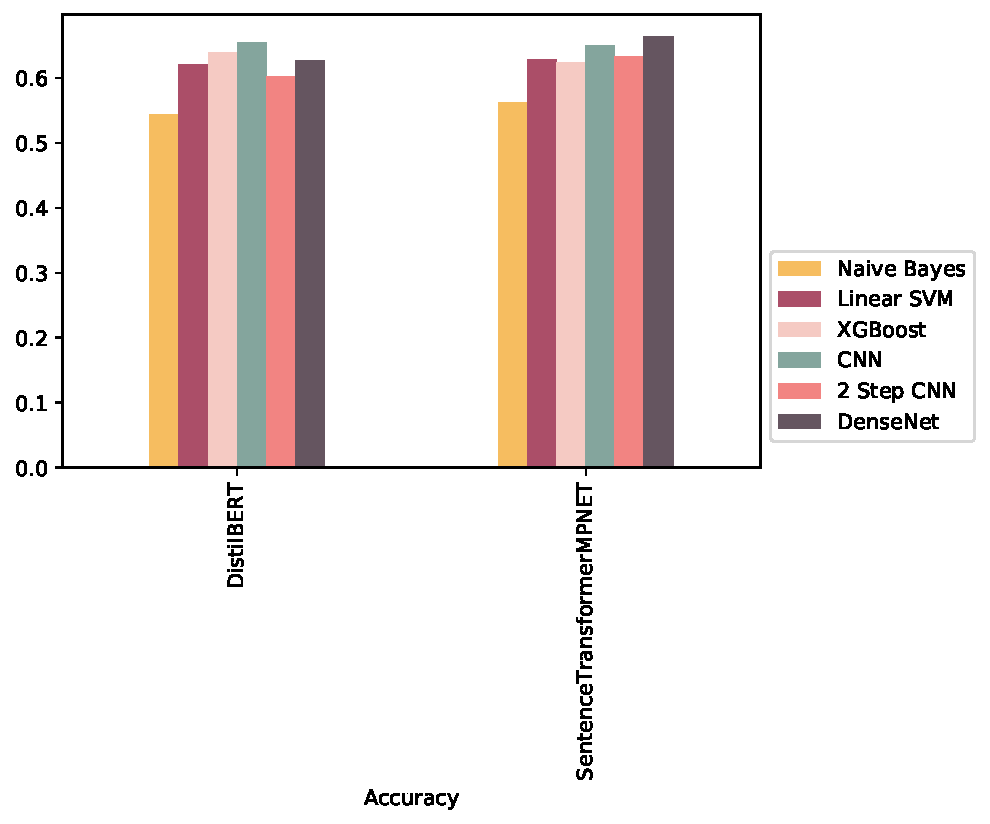
\includegraphics[width=0.8\linewidth]{plots/accuracy_small_balanced.pdf}
\caption{Comparison of DistilBERT and SentenceTransformerMPNET on balanced dataset}
\label{fig:embed_comparison}
\end{figure}


\begin{figure}
\centering
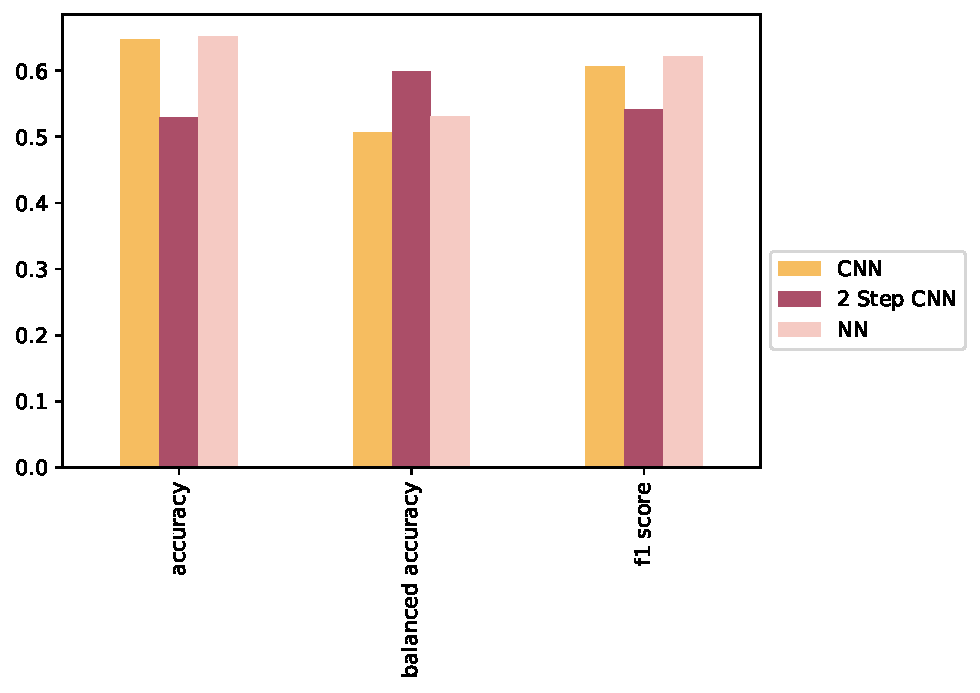
\includegraphics[width=0.8\linewidth]{plots/metrics_comparison_small.pdf}
\caption{Comparison of different metrics for different classifiers on unbalanced dataset}
\label{fig:metric_comparison}
\end{figure}

\begin{table}[h]
\centering
\begin{tabular}{l|l|r|r}
\textbf{Embedding} & \textbf{Classifier} & \textbf{Accuracy} & \textbf{F1 score} \\\hline
Smaller BERT & Naive Bayes & 0.379479 & 0.328668 \\
Smaller BERT & Linear SVM & 0.399837 & 0.353035 \\
Smaller BERT & XGBoost & 0.375407 & 0.374183 \\
Smaller BERT & CNN & 0.415309 & 0.401595 \\
Glove & Naive Bayes & 0.333876 & 0.259667 \\
Glove & Linear SVM & 0.320033 & 0.295821 \\
Glove & XGBoost & 0.343648 & 0.336383 \\
Glove & CNN & 0.374593 & 0.382742 \\
\textbf{DistilBERT} & \textbf{Naive Bayes} & \textbf{0.547231} & \textbf{0.550679} \\
DistilBERT & Linear SVM & 0.477199 & 0.373867 \\
DistilBERT & XGBoost & 0.518730 & 0.519839 \\
DistilBERT & CNN & 0.535016 & 0.530048 \\
DistilBERT & DenseNet & 0.516287 & 0.516995 \\
SentenceTransformerMPNET & CNN & 0.495928 & 0.499407 \\
SentenceTransformerMPNET & DenseNet & 0.517915 & 0.517484 \\
\end{tabular}
\caption{Results for the created dataset and unnormalized lyrics}
\label{tab:dataset_res}
\end{table}

\begin{figure}
\centering
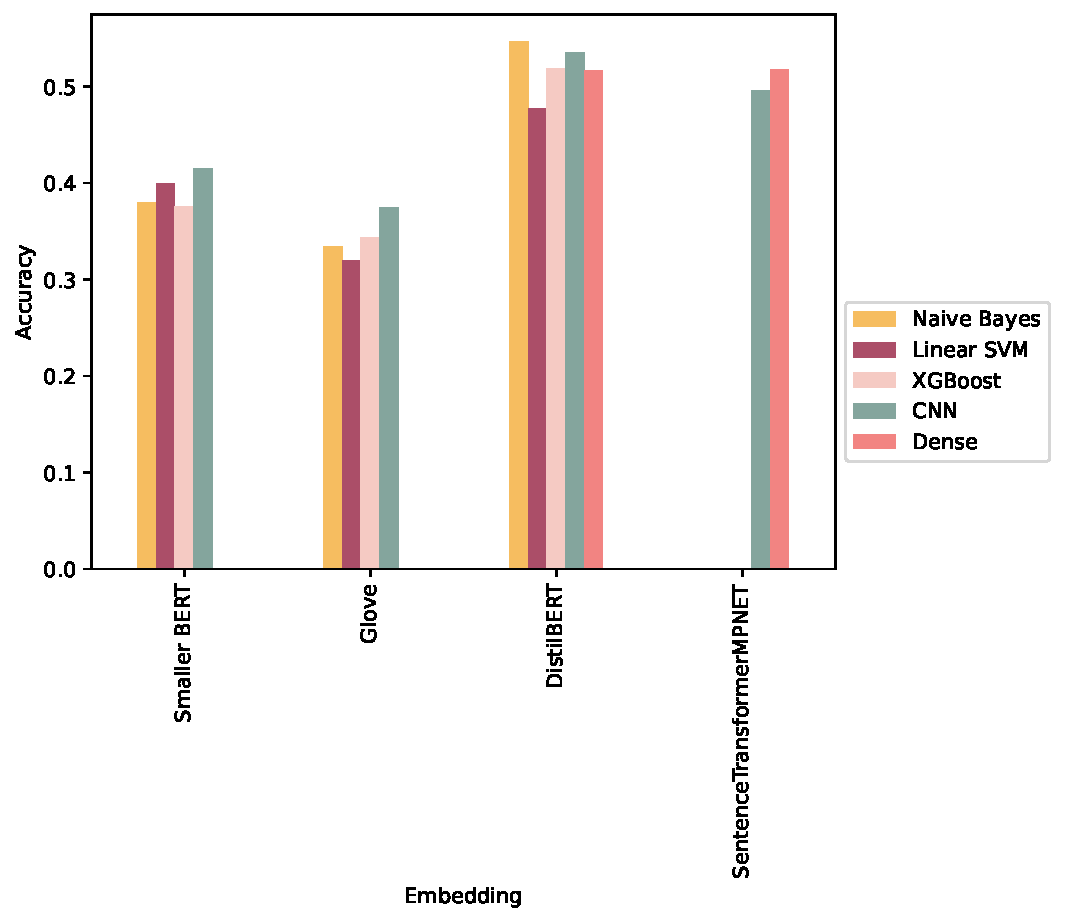
\includegraphics[width=0.8\linewidth]{plots/accuracy_dataset.pdf}
\caption{Accuracy for the created dataset and unnormalized lyrics}
\label{fig:acc_dataset}
\end{figure}

\begin{figure}
\centering
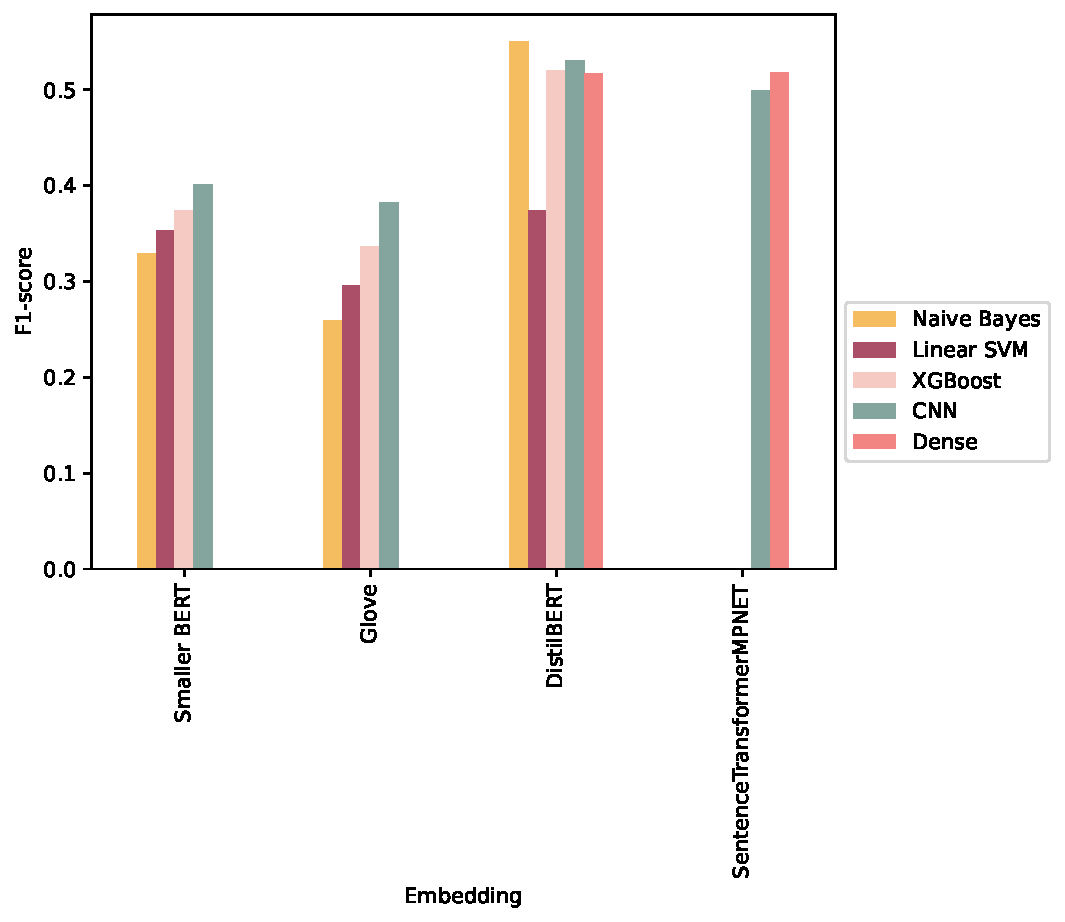
\includegraphics[width=0.8\linewidth]{plots/f1_dataset.pdf}
\caption{F1-score for the created dataset and unnormalized lyrics}
\label{fig:f1_dataset}
\end{figure}

\begin{table}[h]
\centering
\begin{tabular}{l|l|r|r}
\textbf{Embedding} & \textbf{Classifier} & \textbf{Accuracy} & \textbf{F1 score} \\\hline
Smaller BERT & Naive Bayes & 0.310261 & 0.247440 \\
Smaller BERT & Linear SVM & 0.368078 & 0.352763 \\
Smaller BERT & XGBoost & 0.400651 & 0.395027 \\
Smaller BERT & CNN & 0.439739 & 0.439537 \\
Glove & Naive Bayes & 0.328176 & 0.236727 \\
Glove & Linear SVM & 0.383550 & 0.376734 \\
Glove & XGBoost & 0.372964 & 0.369424 \\
Glove & CNN & 0.389251 & 0.395433 \\
DistilBERT & Naive Bayes & 0.515472 & 0.495294 \\
DistilBERT & Linear SVM & \textbf{0.541531} & 0.492267 \\
DistilBERT & XGBoost & 0.503257 & 0.500318 \\
DistilBERT & CNN & 0.494300 & 0.494112 \\
DistilBERT & DenseNet & 0.518730 & \textbf{0.517378} \\
SentenceTransformerMPNET & CNN & 0.514658 & 0.509839 \\
SentenceTransformerMPNET & DenseNet & 0.500000 & 0.501151 \\
\end{tabular}
\caption{Results for the created dataset and normalized lyrics}
\label{tab:dataset_res_norm}
\end{table}

\begin{figure}
\centering
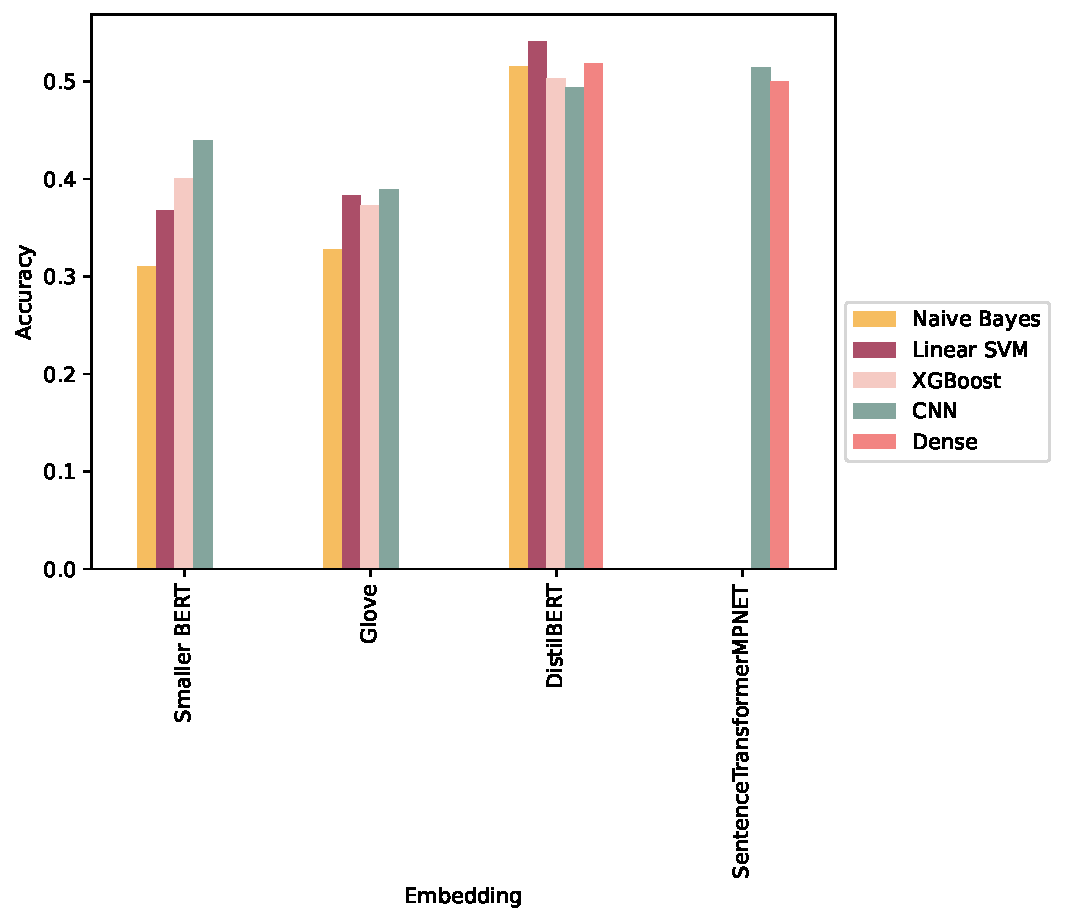
\includegraphics[width=0.8\linewidth]{plots/accuracy_dataset_norm.pdf}
\caption{Accuracy for the created dataset and normalized lyrics}
\label{fig:acc_dataset_norm}
\end{figure}

\begin{figure}
\centering
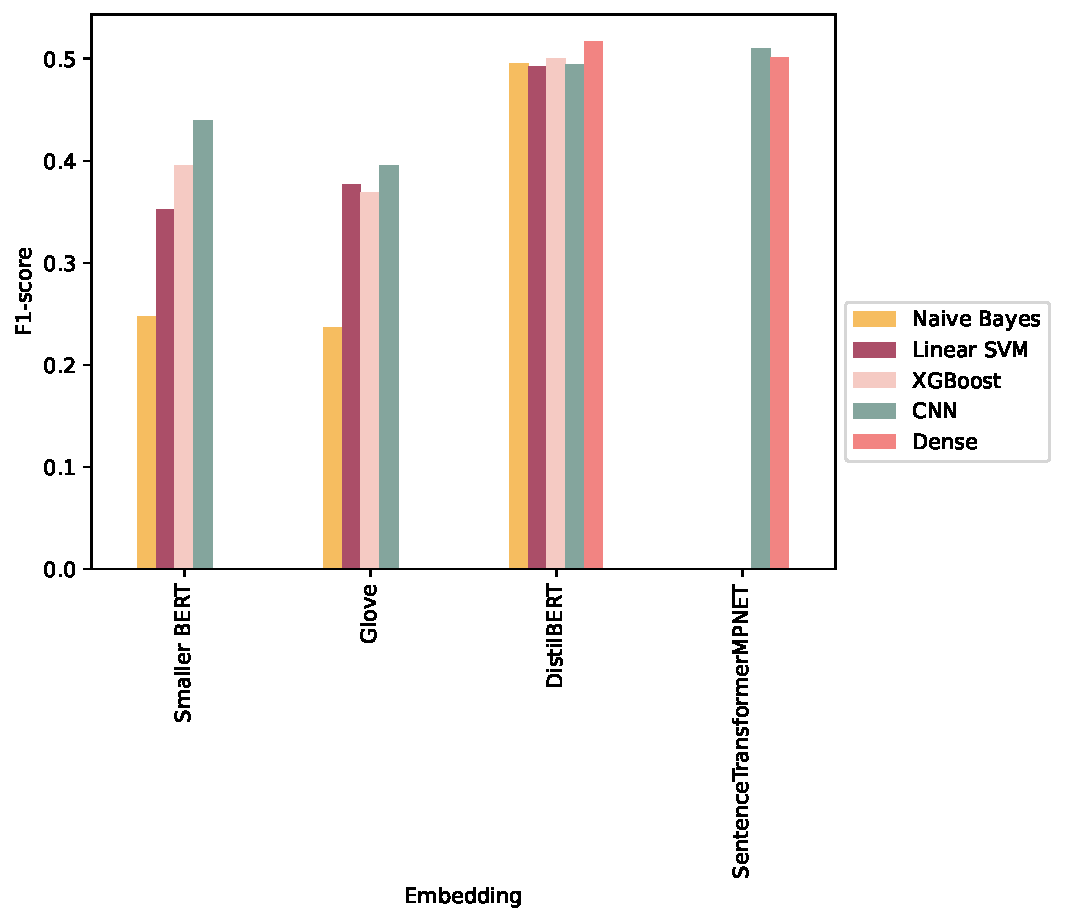
\includegraphics[width=0.8\linewidth]{plots/f1_dataset_norm.pdf}
\caption{F1-score for the created dataset and normalized lyrics}
\label{fig:f1_dataset_norm}
\end{figure}
\twocolumn

\section{Discussion}\label{discussion}
There are several contributions to this work. First of all, we were not able to find a detailed comparison of statistical and deep learning models. Often works focus on a selected group of models like transformers in case of \cite{sig_bert}, 1D CNNs in \cite{audio_1dcnn} or Support Vector Machines explored in \cite{oldAudio}.

What is more, often different datasets are being used, which overall makes the results difficult to compare. Our work compares older and newer models on different datasets. This creates a common ground and context for other works and researchers. When it comes to the comparison of our results to the current state-of-the-art, again the situation is a bit complex. State-of-the-art solution for different, in our opinion simpler, task of genre classification based on audio stands at 80.93\% achieved in \cite{audio_1dcnn}. The best lyrics-based prediction accuracy that we were able to find was 77.63\%, achieved by the BERT model in \cite{sig_bert}.

This cast a strong shadow on our best result of 57.17\% but again, those results are difficult to compare. Why? This is due to the fact that the authors of mentioned SOTA preprocessed the data in an undocumented way, significantly simplifying the original problem present in the dataset. Naturally, as mentioned numerously in this document we also made changes to the formulation of the original problem, but due to the missing information from other works we are not able to reproduce this process in a similar way, hence making the results non-conclusive. What is worse, the mentioned article makes use of a different dataset, which makes the accuracy even harder to compare. 



\section{Conclusion}\label{conclusion}

Music genre classification performance seems to be limited strictly by the lyrics embedding quality. The most significant improvements were observed when switching to embedding models with substantially different complexity. This suggests that further improvements in this field may be achieved just by scaling up the embedding models. 
On the other hand, the typical procedure of fine-tuning pre-trained general language models, done  on presented music genre data, did not bring significant improvements when compared to using just pre-trained models.

Fusing lyrics data, in the form of embeddings, with the sentiment of the lyrics did not bring significant improvements when tested in different settings.

The fusion of two models in the form of a 2-step classifier gives better results when it comes to balanced accuracy but worse overall. The problem may be that errors from the two models accumulate when they are used together. However, this approach can still be useful depending on the task at hand.

In the case of small datasets, simpler classifiers may give better results and are faster than training e.g. CNNs for multiple epochs.
 


\printbibliography

\end{document}


